%!TEX program = xelatex
\documentclass[12pt,a4paper]{report}
\usepackage[utf8]{inputenc}
\usepackage[margin=1in]{geometry}
\usepackage{hyperref}
\usepackage{graphicx}
\usepackage{xcolor}
\usepackage{tikz}
\usepackage{tcolorbox}
\usepackage{listings}
\usepackage{fontawesome5}
\usepackage{booktabs}
\usepackage{enumitem}
\usepackage{amsmath}
\usepackage{fancyhdr}
\usepackage{titlesec}

\usetikzlibrary{shapes,arrows,positioning,shadows,backgrounds,fit,calc}

% Color definitions
\definecolor{primary}{RGB}{59,130,246}
\definecolor{secondary}{RGB}{147,51,234}
\definecolor{success}{RGB}{34,197,94}
\definecolor{warning}{RGB}{234,179,8}
\definecolor{danger}{RGB}{239,68,68}
\definecolor{codebg}{RGB}{248,250,252}

% Hyperref setup
\hypersetup{
    colorlinks=true,
    linkcolor=primary,
    filecolor=secondary,
    urlcolor=primary,
    citecolor=success,
    pdfauthor={Ayush Pandey},
    pdftitle={Momentum - AI-Powered Productivity Platform},
    pdfsubject={Technical Documentation},
    pdfkeywords={productivity, AI, time management, gamification}
}

% Custom title formatting
\titleformat{\chapter}[display]
{\normalfont\huge\bfseries\color{primary}}
{\chaptertitlename\ \thechapter}{20pt}{\Huge}

\titleformat{\section}
{\normalfont\Large\bfseries\color{primary}}
{\thesection}{1em}{}

\titleformat{\subsection}
{\normalfont\large\bfseries\color{secondary}}
{\thesubsection}{1em}{}

% Headers and footers
\pagestyle{fancy}
\fancyhf{}
\fancyhead[L]{\leftmark}
\fancyhead[R]{Momentum Platform}
\fancyfoot[C]{\thepage}
\renewcommand{\headrulewidth}{2pt}
\renewcommand{\footrulewidth}{1pt}

% Code listing setup
\lstset{
    basicstyle=\ttfamily\small,
    backgroundcolor=\color{codebg},
    breaklines=true,
    frame=single,
    numbers=left,
    numberstyle=\tiny\color{gray},
    keywordstyle=\color{primary}\bfseries,
    commentstyle=\color{success},
    stringstyle=\color{danger},
    showstringspaces=false,
    tabsize=2
}

% Custom boxes
\newtcolorbox{featurebox}[1]{
    colback=primary!5,
    colframe=primary,
    fonttitle=\bfseries,
    title=#1,
    boxrule=2pt,
    arc=4pt
}

\newtcolorbox{techbox}[1]{
    colback=secondary!5,
    colframe=secondary,
    fonttitle=\bfseries,
    title=#1,
    boxrule=2pt,
    arc=4pt
}

\newtcolorbox{notebox}{
    colback=warning!10,
    colframe=warning,
    boxrule=2pt,
    arc=4pt
}

% Title page
\begin{document}

\begin{titlepage}
    \centering
    \vspace*{2cm}
    
    {\Huge\bfseries\color{primary} MOMENTUM\par}
    \vspace{0.5cm}
    {\Large AI-Powered Time Management \& Productivity Platform\par}
    \vspace{2cm}
    
    % TikZ logo/icon
    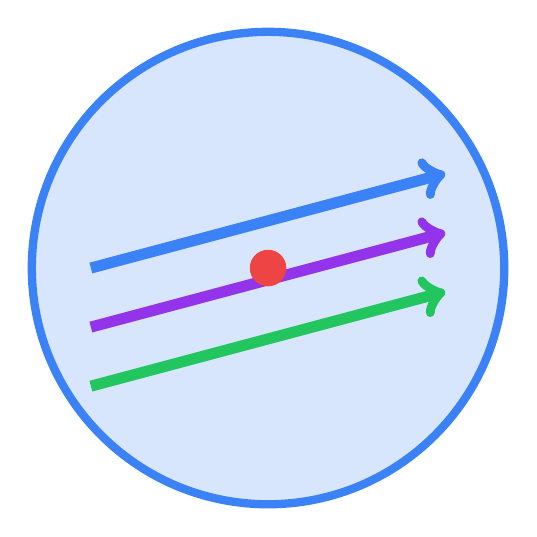
\begin{tikzpicture}[scale=1.5]
        % Main circle
        \draw[fill=primary!20, draw=primary, line width=3pt] (0,0) circle (2);
        
        % Momentum arrow
        \draw[->, line width=4pt, primary] (-1.5,0) -- (1.5,0.8);
        \draw[->, line width=4pt, secondary] (-1.5,-0.5) -- (1.5,0.3);
        \draw[->, line width=4pt, success] (-1.5,-1) -- (1.5,-0.2);
        
        % Center dot
        \draw[fill=danger, draw=danger] (0,0) circle (0.15);
    \end{tikzpicture}
    
    \vspace{2cm}
    {\Large\bfseries Comprehensive Technical Documentation\par}
    \vspace{1cm}
    
    {\large Version 1.0\par}
    \vspace{0.5cm}
    {\large \today\par}
    
    \vfill
    
    {\large\bfseries Author\par}
    {\large Ayush Pandey\par}
    \vspace{0.3cm}
    {\large\faGithub\ \href{https://github.com/AyushPandey003}{github.com/AyushPandey003}\par}
    
\end{titlepage}

\tableofcontents

% Abstract
\chapter*{Abstract}
\addcontentsline{toc}{chapter}{Abstract}

\textbf{Momentum} is a cutting-edge AI-powered time management and productivity platform designed for students, professionals, and anyone seeking to optimize their daily workflow. By combining intelligent task decomposition, automated scheduling, gamification mechanics, and real-time competitive features, Momentum transforms how users approach productivity and time management.

\vspace{0.5cm}

The platform leverages modern web technologies including Next.js 14, React Server Components, Drizzle ORM with PostgreSQL, and WebSocket-based real-time communication to deliver a seamless, responsive user experience. Advanced AI capabilities powered by Google's Gemini model enable intelligent task breakdown and personalized productivity coaching.

\vspace{0.5cm}

Key innovations include:
\begin{itemize}
    \item \textbf{AI Task Decomposition} - Automatically breaks complex tasks into manageable subtasks
    \item \textbf{Intelligent Scheduling} - Smart time-blocking with Pomodoro integration
    \item \textbf{Real-time Contests} - Competitive knowledge challenges with friends
    \item \textbf{Gamification Engine} - Achievements, levels, and leaderboards
    \item \textbf{Wellness Integration} - Automated break reminders and health tracking
    \item \textbf{Manager Verification} - Task accountability through email verification
\end{itemize}

% Chapter 1: Introduction
\chapter{Introduction}

\section{Overview}

Momentum addresses the universal challenge of productivity management by providing an intelligent, adaptive system that understands user behavior and optimizes task completion. Unlike traditional to-do list applications, Momentum actively coaches users, prevents procrastination, and makes productivity engaging through game mechanics.

\section{Problem Statement}

Modern professionals and students face several productivity challenges:
\begin{enumerate}
    \item \textbf{Task Overwhelm} - Large projects appear insurmountable
    \item \textbf{Poor Time Estimation} - Difficulty accurately estimating task duration
    \item \textbf{Procrastination Patterns} - Unconscious avoidance of difficult tasks
    \item \textbf{Lack of Accountability} - No external verification of task completion
    \item \textbf{Motivation Decay} - Difficulty maintaining long-term productivity habits
\end{enumerate}

\section{Solution Architecture}

Momentum employs a multi-layered architecture to address these challenges:

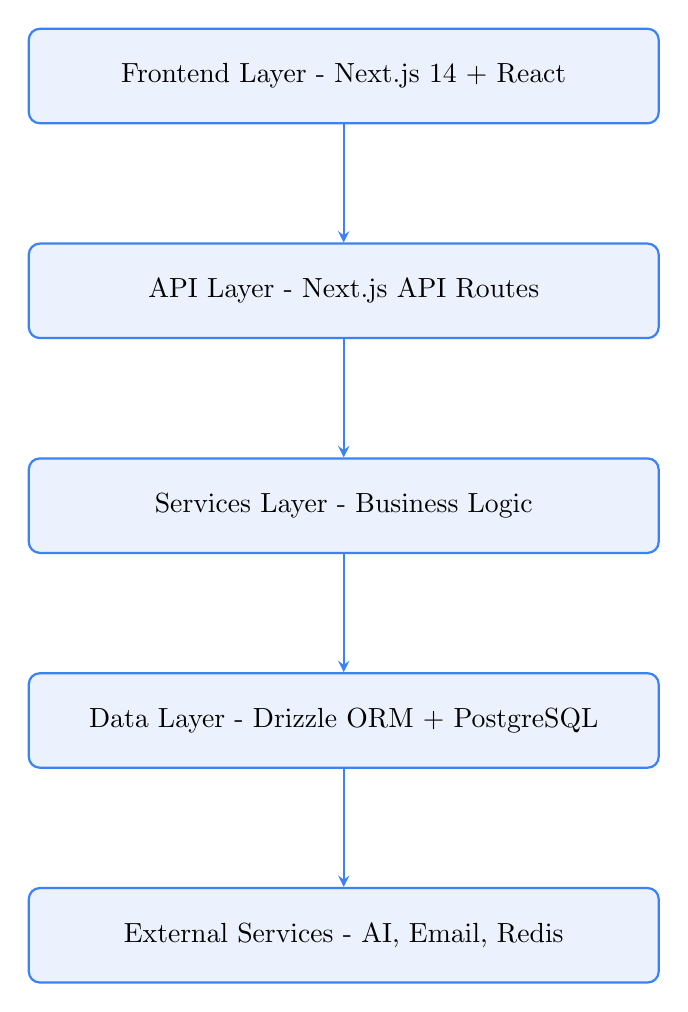
\begin{tikzpicture}[
    node distance=1.5cm,
    layer/.style={rectangle, draw=primary, fill=primary!10, thick, minimum width=8cm, minimum height=1.2cm, text centered, rounded corners},
    arrow/.style={->, >=stealth, thick, primary}
]
    % Layers
    \node[layer] (frontend) {Frontend Layer - Next.js 14 + React};
    \node[layer, below=of frontend] (api) {API Layer - Next.js API Routes};
    \node[layer, below=of api] (services) {Services Layer - Business Logic};
    \node[layer, below=of services] (data) {Data Layer - Drizzle ORM + PostgreSQL};
    \node[layer, below=of data] (external) {External Services - AI, Email, Redis};
    
    % Arrows
    \draw[arrow] (frontend) -- (api);
    \draw[arrow] (api) -- (services);
    \draw[arrow] (services) -- (data);
    \draw[arrow] (data) -- (external);
\end{tikzpicture}

\section{Technology Stack}

\begin{featurebox}{Frontend Technologies}
\begin{itemize}
    \item \textbf{Next.js 14} - React framework with App Router and Server Components
    \item \textbf{TypeScript} - Type-safe development environment
    \item \textbf{Tailwind CSS} - Utility-first CSS framework
    \item \textbf{Radix UI} - Accessible component primitives
    \item \textbf{Shadcn/ui} - Beautiful, customizable UI components
\end{itemize}
\end{featurebox}

\begin{techbox}{Backend Technologies}
\begin{itemize}
    \item \textbf{Next.js API Routes} - Serverless API endpoints
    \item \textbf{Better Auth} - Modern authentication solution
    \item \textbf{Drizzle ORM} - Type-safe SQL ORM
    \item \textbf{PostgreSQL (Neon)} - Serverless PostgreSQL database
    \item \textbf{Upstash Redis} - Serverless Redis for caching and rate limiting
\end{itemize}
\end{techbox}

\begin{featurebox}{AI \& External Services}
\begin{itemize}
    \item \textbf{Google Gemini AI} - Task decomposition and AI mentoring
    \item \textbf{Gmail API} - Email notifications and invitations
    \item \textbf{UploadThing} - File upload and storage
    \item \textbf{React Email} - Beautiful transactional emails
\end{itemize}
\end{featurebox}

% Chapter 2: Core Features
\chapter{Core Features}

\section{AI-Powered Task Decomposition}

\subsection{Overview}
The task decomposition engine uses Google's Gemini AI model to analyze complex tasks and break them into manageable subtasks with estimated time allocations.

\subsection{Technical Implementation}

\begin{lstlisting}[language=JavaScript, caption=AI Task Decomposition Service]
// lib/ai.ts
import { GoogleGenerativeAI } from "@google/generative-ai";

const genAI = new GoogleGenerativeAI(
    process.env.GOOGLE_GEMINI_API_KEY!
);

export async function decomposeTask(taskDescription: string) {
    const model = genAI.getGenerativeModel({ 
        model: "gemini-1.5-flash" 
    });
    
    const prompt = `Break down this task into subtasks...`;
    const result = await model.generateContent(prompt);
    return parseSubtasks(result.response.text());
}
\end{lstlisting}

\subsection{Algorithm Flow}

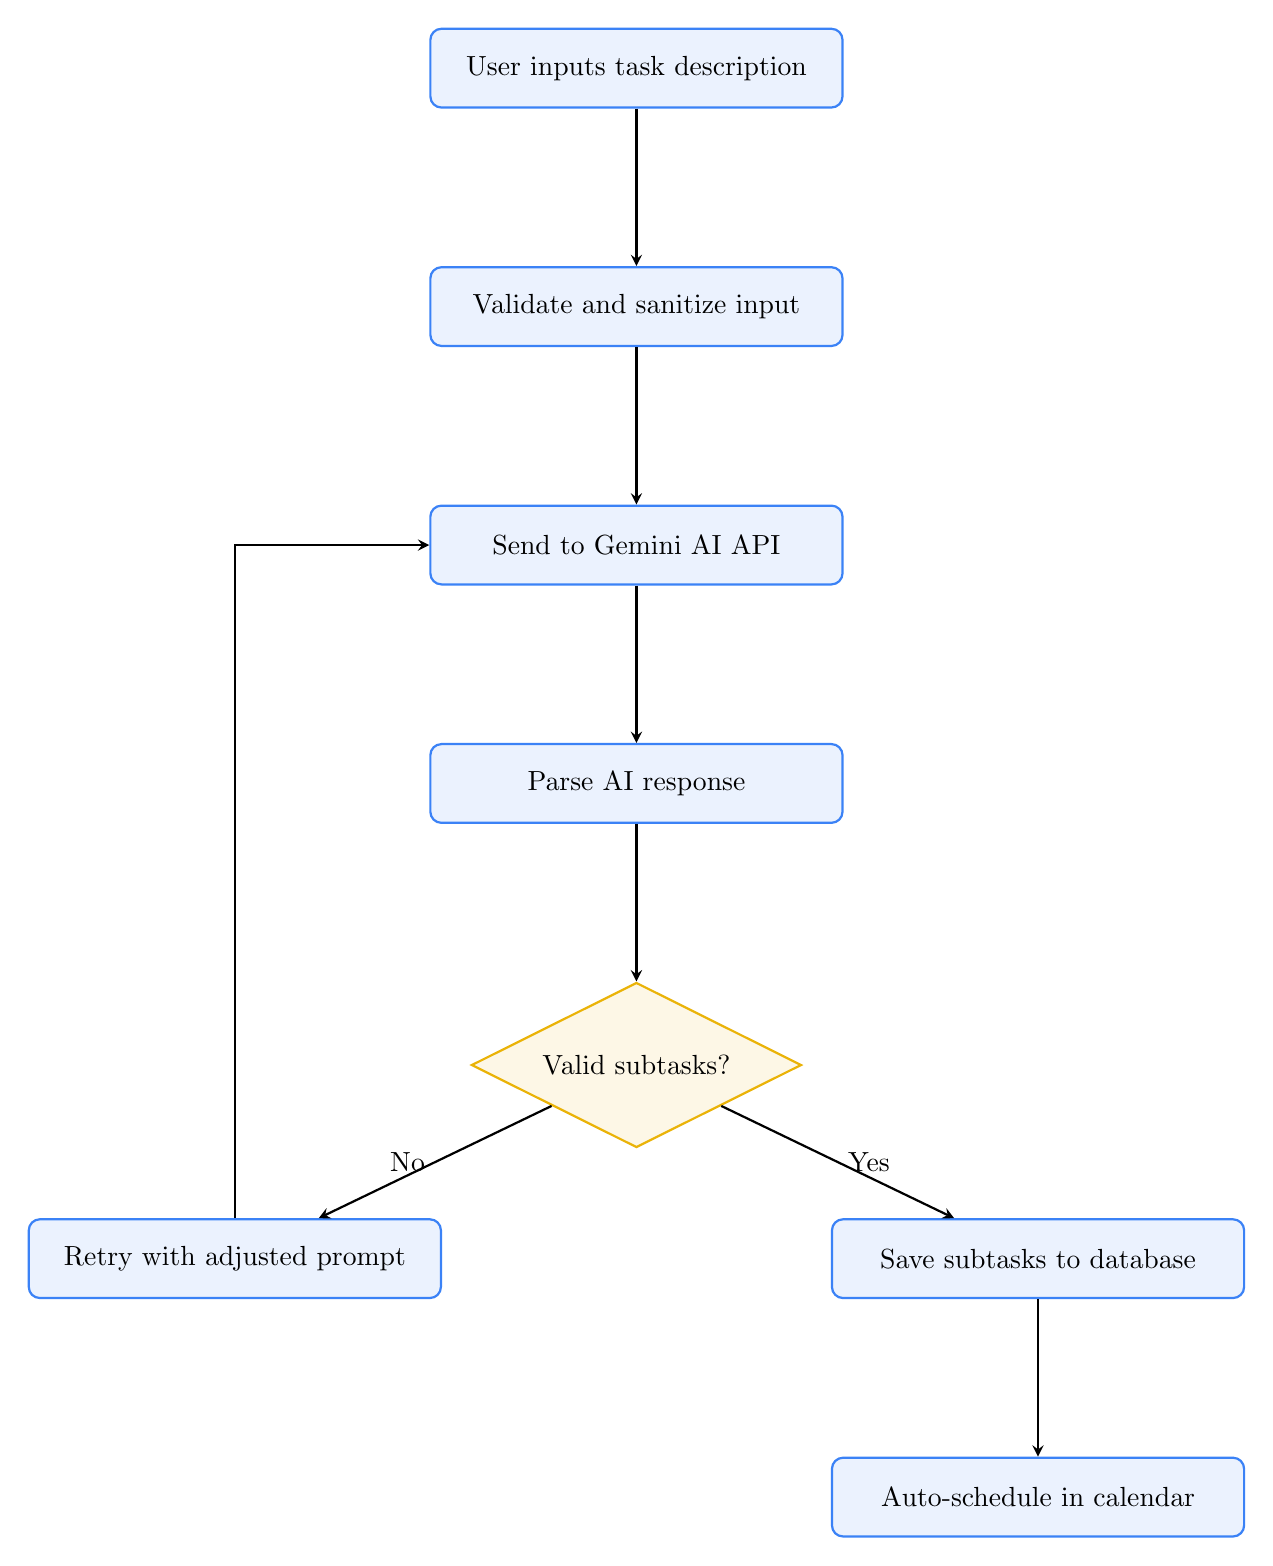
\begin{tikzpicture}[
    node distance=2cm,
    process/.style={rectangle, draw=primary, fill=primary!10, thick, text width=5cm, text centered, rounded corners, minimum height=1cm},
    decision/.style={diamond, draw=warning, fill=warning!10, thick, text width=3cm, text centered, aspect=2},
    arrow/.style={->, >=stealth, thick}
]
    \node[process] (input) {User inputs task description};
    \node[process, below=of input] (validate) {Validate and sanitize input};
    \node[process, below=of validate] (ai) {Send to Gemini AI API};
    \node[process, below=of ai] (parse) {Parse AI response};
    \node[decision, below=of parse] (check) {Valid subtasks?};
    \node[process, below left=of check] (retry) {Retry with adjusted prompt};
    \node[process, below right=of check] (save) {Save subtasks to database};
    \node[process, below=of save] (schedule) {Auto-schedule in calendar};
    
    \draw[arrow] (input) -- (validate);
    \draw[arrow] (validate) -- (ai);
    \draw[arrow] (ai) -- (parse);
    \draw[arrow] (parse) -- (check);
    \draw[arrow] (check) -- node[anchor=east] {No} (retry);
    \draw[arrow] (retry) |- (ai);
    \draw[arrow] (check) -- node[anchor=west] {Yes} (save);
    \draw[arrow] (save) -- (schedule);
\end{tikzpicture}

\subsection{Subtask Schema}

Each generated subtask contains:
\begin{itemize}
    \item \textbf{Title} - Clear, actionable description
    \item \textbf{Estimated Time} - AI-predicted duration in minutes
    \item \textbf{Priority} - Relative importance (low, medium, high, urgent)
    \item \textbf{Dependencies} - Sequential ordering if required
    \item \textbf{Completion Status} - Boolean tracking
\end{itemize}

\section{Intelligent Scheduling System}

\subsection{Pomodoro Integration}

The scheduler integrates the Pomodoro Technique with intelligent time-blocking:

\[
\text{Pomodoro Session} = \begin{cases}
    \text{Focus Block} & : 25 \text{ minutes (default)} \\
    \text{Short Break} & : 5 \text{ minutes} \\
    \text{Long Break} & : 15 \text{ minutes (every 4 sessions)}
\end{cases}
\]

\subsection{Schedule Block Types}

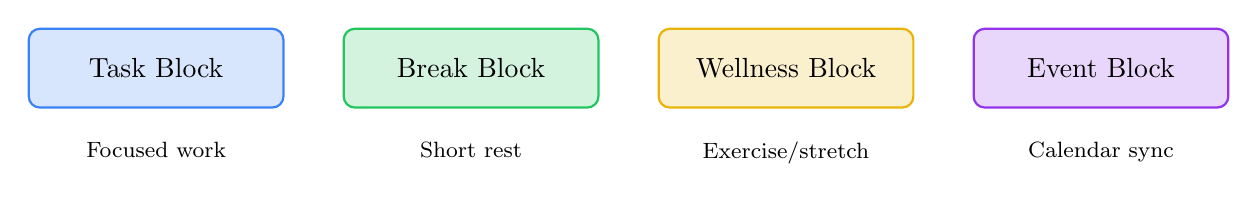
\begin{tikzpicture}[
    block/.style={rectangle, draw, thick, text width=3cm, text centered, minimum height=1cm, rounded corners},
    task/.style={block, fill=primary!20, draw=primary},
    break/.style={block, fill=success!20, draw=success},
    wellness/.style={block, fill=warning!20, draw=warning},
    event/.style={block, fill=secondary!20, draw=secondary}
]
    \node[task] (t1) at (0,0) {Task Block};
    \node[break] (b1) at (4,0) {Break Block};
    \node[wellness] (w1) at (8,0) {Wellness Block};
    \node[event] (e1) at (12,0) {Event Block};
    
    \node[below=0.3cm of t1] {\footnotesize Focused work};
    \node[below=0.3cm of b1] {\footnotesize Short rest};
    \node[below=0.3cm of w1] {\footnotesize Exercise/stretch};
    \node[below=0.3cm of e1] {\footnotesize Calendar sync};
\end{tikzpicture}

\subsection{Auto-Scheduling Algorithm}

\begin{notebox}
The scheduler considers:
\begin{enumerate}
    \item User-defined work hours (default: 9 AM - 5 PM)
    \item Task priority and deadlines
    \item Estimated task duration
    \item Existing calendar commitments
    \item Mandatory wellness breaks every 30 minutes
    \item User's historical productivity patterns
\end{enumerate}
\end{notebox}

\section{Procrastination Detection \& Prevention}

\subsection{Detection Mechanisms}

The system monitors for procrastination patterns:

\begin{enumerate}
    \item \textbf{Deadline Approaching} - Task due within 24 hours but not started
    \item \textbf{Task Avoidance} - High-priority task skipped multiple times
    \item \textbf{Pattern Detection} - Consistent delays on specific task types
\end{enumerate}

\subsection{Alert Severity Levels}

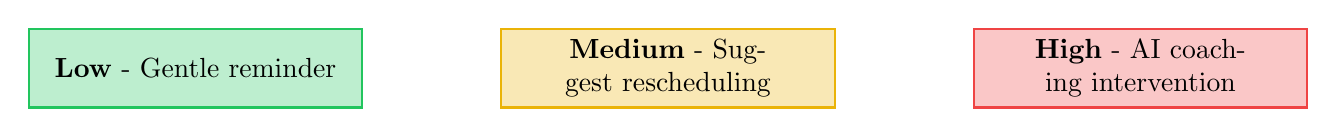
\begin{tikzpicture}[
    level/.style={rectangle, draw, thick, text width=4cm, text centered, minimum height=1cm},
    low/.style={level, fill=success!30, draw=success},
    medium/.style={level, fill=warning!30, draw=warning},
    high/.style={level, fill=danger!30, draw=danger}
]
    \node[low] (l) at (0,0) {\textbf{Low} - Gentle reminder};
    \node[medium] (m) at (6,0) {\textbf{Medium} - Suggest rescheduling};
    \node[high] (h) at (12,0) {\textbf{High} - AI coaching intervention};
\end{tikzpicture}

\section{Gamification System}

\subsection{Points \& Experience}

Users earn points through various activities:

\begin{table}[h]
\centering
\begin{tabular}{@{}lcc@{}}
\toprule
\textbf{Activity} & \textbf{Points} & \textbf{XP} \\ \midrule
Complete Task & 10-50 & 10-50 \\
Complete Pomodoro & 5 & 5 \\
Maintain Streak & 20/day & 20/day \\
Unlock Achievement & Varies & Varies \\
Win Contest & 100 & 100 \\
\bottomrule
\end{tabular}
\caption{Points and XP earning system}
\end{table}

\subsection{Level Progression Formula}

The level calculation uses a square root scaling function:

\[
\text{Level} = \lfloor\sqrt{\frac{\text{Total Points}}{100}}\rfloor + 1
\]

Points required for next level:
\[
\text{Points}_{\text{next}} = \text{Current Level}^2 \times 100
\]

\subsection{Achievement System}

\begin{featurebox}{Achievement Categories}
\begin{itemize}
    \item \textbf{Task Achievements} - Complete 1, 10, 50, 100 tasks
    \item \textbf{Pomodoro Achievements} - Focus mastery milestones
    \item \textbf{Streak Achievements} - Consistency rewards (3, 7, 30 days)
    \item \textbf{Contest Achievements} - Competition participation and victories
    \item \textbf{Special Achievements} - Unique accomplishments
\end{itemize}
\end{featurebox}

\section{Contest System}

\subsection{Contest Architecture}

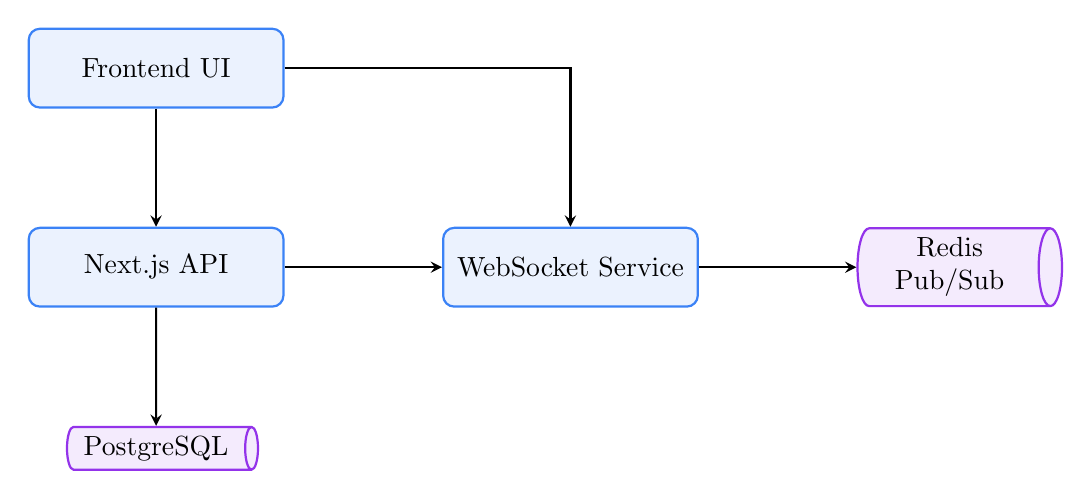
\begin{tikzpicture}[
    node distance=1.5cm and 2cm,
    component/.style={rectangle, draw=primary, fill=primary!10, thick, text width=3cm, text centered, rounded corners, minimum height=1cm},
    database/.style={cylinder, draw=secondary, fill=secondary!10, thick, aspect=0.3, text width=2cm, text centered},
    arrow/.style={->, >=stealth, thick}
]
    \node[component] (frontend) {Frontend UI};
    \node[component, below=of frontend] (api) {Next.js API};
    \node[database, below=of api] (db) {PostgreSQL};
    \node[component, right=of api] (ws) {WebSocket Service};
    \node[database, right=of ws] (redis) {Redis Pub/Sub};
    
    \draw[arrow] (frontend) -- (api);
    \draw[arrow] (api) -- (db);
    \draw[arrow] (frontend) -| (ws);
    \draw[arrow] (ws) -- (redis);
    \draw[arrow] (api) -- (ws);
\end{tikzpicture}

\subsection{Contest Types}

\begin{enumerate}
    \item \textbf{Quick Fire} (15 min) - Fast-paced, 10 questions
    \item \textbf{Standard} (30 min) - Balanced competition
    \item \textbf{Marathon} (60 min) - Endurance challenge
\end{enumerate}

\subsection{Contest Flow State Machine}

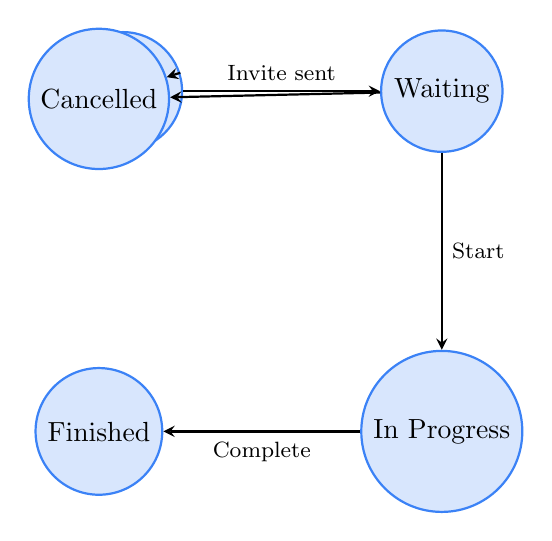
\begin{tikzpicture}[
    node distance=2.5cm,
    state/.style={circle, draw=primary, fill=primary!20, thick, text centered, minimum size=1.5cm},
    arrow/.style={->, >=stealth, thick}
]
    \node[state] (draft) {Draft};
    \node[state, right=of draft] (waiting) {Waiting};
    \node[state, below=of waiting] (progress) {In Progress};
    \node[state, left=of progress] (finished) {Finished};
    \node[state, above=of finished] (cancelled) {Cancelled};
    
    \draw[arrow] (draft) -- node[above] {\footnotesize Invite sent} (waiting);
    \draw[arrow] (waiting) -- node[right] {\footnotesize Start} (progress);
    \draw[arrow] (progress) -- node[below] {\footnotesize Complete} (finished);
    \draw[arrow] (draft) -- (cancelled);
    \draw[arrow] (waiting) -- (cancelled);
\end{tikzpicture}

\subsection{Real-time Scoring Algorithm}

Scoring considers both accuracy and speed:

\[
\text{Points} = \text{Base Points} \times \left(1 + \frac{\text{Time Remaining}}{\text{Total Time}} \times 0.5\right)
\]

Where:
\begin{itemize}
    \item Base Points = 10 (configurable per question)
    \item Time bonus up to 50\% of base points
    \item Faster correct answers earn more points
\end{itemize}

\section{Wellness \& Health Integration}

\subsection{Wellness Metrics}

The platform tracks four key wellness dimensions:

\begin{tikzpicture}[scale=0.8]
    % Create 4 quadrants for wellness metrics
    \draw[draw=primary, thick] (-3,0) -- (3,0);
    \draw[draw=primary, thick] (0,-3) -- (0,3);
    
    % Quadrant labels
    \node[text=primary, font=\bfseries] at (-1.5, 1.5) {Hydration};
    \node[text=secondary, font=\bfseries] at (1.5, 1.5) {Breaks};
    \node[text=success, font=\bfseries] at (-1.5, -1.5) {Eye Rest};
    \node[text=warning, font=\bfseries] at (1.5, -1.5) {Movement};
    
    % Icons (simplified)
    \node at (-1.5, 0.8) {\Large \faGlassWater};
    \node at (1.5, 0.8) {\Large \faClock};
    \node at (-1.5, -0.8) {\Large \faEye};
    \node at (1.5, -0.8) {\Large \faWalking};
    
    % Goals
    \node[font=\small] at (-1.5, -2.3) {Goal: 8 glasses/day};
    \node[font=\small] at (1.5, -2.3) {Goal: 3 sessions/day};
\end{tikzpicture}

\subsection{Reminder System}

Automatic reminders based on activity patterns:
\begin{itemize}
    \item \textbf{Every 30 min} - Stand and stretch reminder
    \item \textbf{Every 60 min} - Hydration reminder
    \item \textbf{Every 20 min} - 20-20-20 eye rest rule
    \item \textbf{Configurable} - User preferences override defaults
\end{itemize}

\section{Manager Verification System}

\subsection{Workflow}

\begin{tikzpicture}[
    node distance=1.8cm,
    step/.style={rectangle, draw=primary, fill=primary!10, thick, text width=4cm, text centered, rounded corners, minimum height=1cm},
    arrow/.style={->, >=stealth, thick}
]
    \node[step] (create) {User creates task};
    \node[step, below=of create] (assign) {Assigns manager email};
    \node[step, below=of assign] (email) {System sends verification email};
    \node[step, below=of email] (complete) {User completes task};
    \node[step, below=of complete] (upload) {Uploads verification image};
    \node[step, below=of upload] (manager) {Manager reviews \& confirms};
    \node[step, below=of manager] (reward) {Points awarded};
    
    \draw[arrow] (create) -- (assign);
    \draw[arrow] (assign) -- (email);
    \draw[arrow] (email) -- (complete);
    \draw[arrow] (complete) -- (upload);
    \draw[arrow] (upload) -- (manager);
    \draw[arrow] (manager) -- (reward);
\end{tikzpicture}

\subsection{Security Measures}

\begin{notebox}
\textbf{Verification Token System:}
\begin{itemize}
    \item Unique cryptographic tokens per task
    \item Token expiration (7 days default)
    \item One-time use validation
    \item Email domain verification
    \item Image upload validation via UploadThing
\end{itemize}
\end{notebox}

% Chapter 3: Database Architecture
\chapter{Database Architecture}

\section{Schema Overview}

The database uses PostgreSQL with Drizzle ORM for type-safe queries. The schema consists of 20+ tables organized into logical domains.

\section{Entity Relationship Diagram}

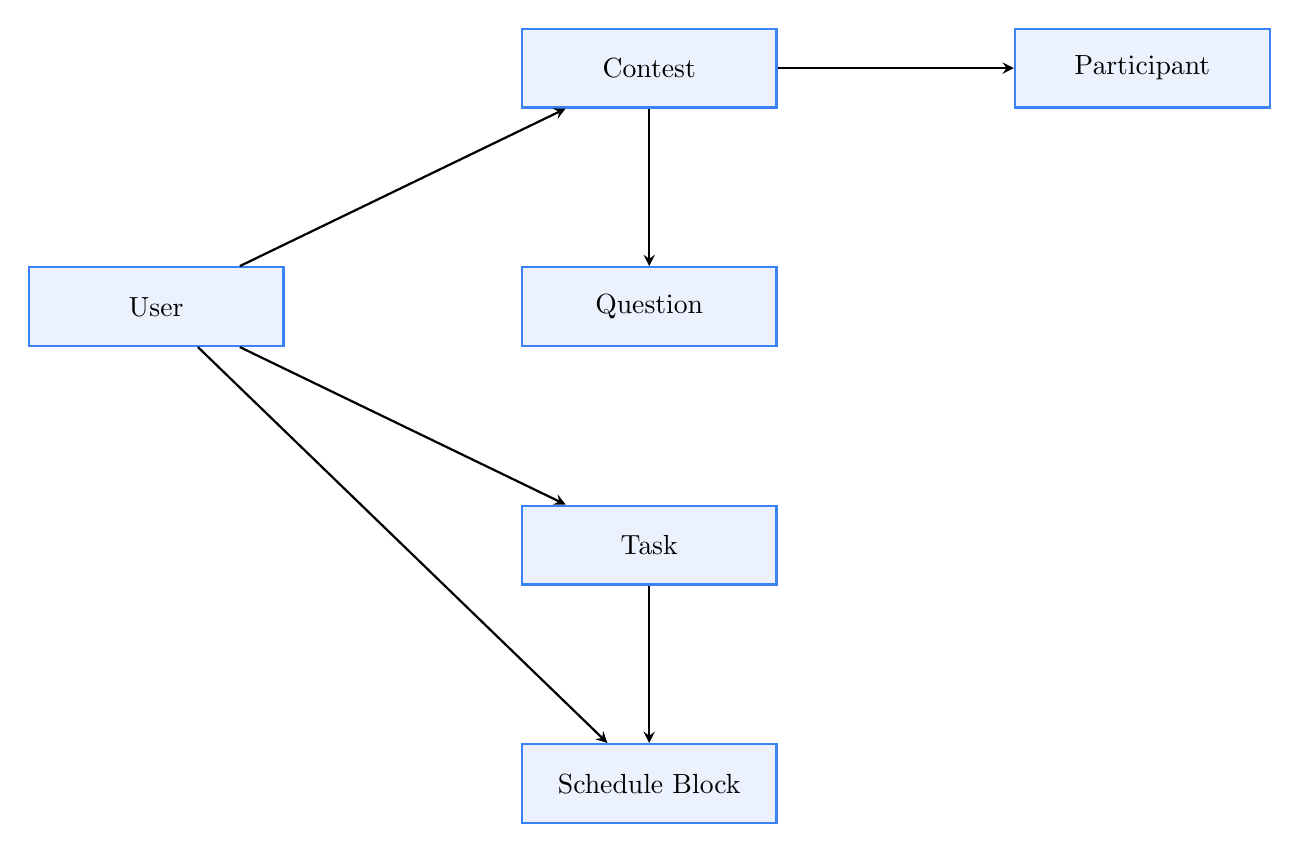
\begin{tikzpicture}[
    node distance=2cm and 3cm,
    entity/.style={rectangle, draw=primary, fill=primary!10, thick, text width=3cm, minimum height=1cm, text centered},
    relation/.style={diamond, draw=secondary, fill=secondary!10, thick, text width=2cm, aspect=2, text centered},
    arrow/.style={->, >=stealth, thick}
]
    % Core entities
    \node[entity] (user) {User};
    \node[entity, below right=of user] (task) {Task};
    \node[entity, above right=of user] (contest) {Contest};
    \node[entity, below=of task] (schedule) {Schedule Block};
    \node[entity, right=of contest] (participant) {Participant};
    \node[entity, below=of contest] (question) {Question};
    
    % Relationships
    \draw[arrow] (user) -- (task);
    \draw[arrow] (user) -- (contest);
    \draw[arrow] (user) -- (schedule);
    \draw[arrow] (contest) -- (participant);
    \draw[arrow] (contest) -- (question);
    \draw[arrow] (task) -- (schedule);
\end{tikzpicture}

\section{Core Tables}

\subsection{User Table}

\begin{lstlisting}[language=SQL, caption=User Schema]
CREATE TABLE "user" (
    id TEXT PRIMARY KEY,
    name TEXT NOT NULL,
    email TEXT NOT NULL UNIQUE,
    email_verified BOOLEAN DEFAULT false,
    image TEXT,
    created_at TIMESTAMP DEFAULT NOW(),
    updated_at TIMESTAMP DEFAULT NOW()
);
\end{lstlisting}

\subsection{Task Table}

\begin{featurebox}{Task Schema Fields}
\begin{itemize}
    \item \texttt{id} - Unique identifier (ULID)
    \item \texttt{userId} - Foreign key to user
    \item \texttt{title} - Task description
    \item \texttt{description} - Detailed information
    \item \texttt{dueDate} - Deadline (ISO 8601)
    \item \texttt{priority} - ENUM: low | medium | high | urgent
    \item \texttt{status} - ENUM: todo | in-progress | completed | overdue
    \item \texttt{estimatedTime} - Duration in minutes
    \item \texttt{actualTime} - Tracked completion time
    \item \texttt{subtasks} - JSON array of subtasks
    \item \texttt{aiDecomposed} - Boolean flag
    \item \texttt{managerEmail} - Verification manager
    \item \texttt{verificationImageUrl} - Proof of completion
\end{itemize}
\end{featurebox}

\subsection{Contest Tables}

The contest system uses 7 interconnected tables:

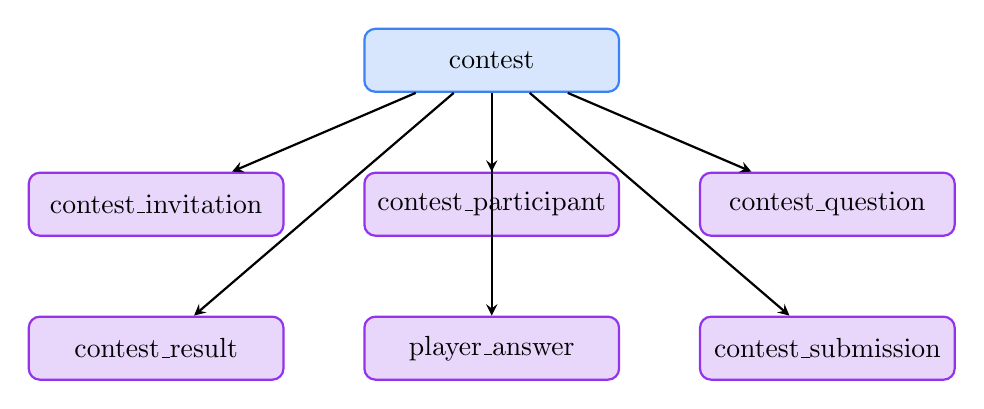
\begin{tikzpicture}[
    table/.style={rectangle, draw, thick, text width=3cm, text centered, minimum height=0.8cm, rounded corners},
    main/.style={table, fill=primary!20, draw=primary},
    sub/.style={table, fill=secondary!20, draw=secondary},
    arrow/.style={->, >=stealth, thick}
]
    \node[main] (contest) {contest};
    \node[sub, below left=1cm and 1cm of contest] (invitation) {contest\_invitation};
    \node[sub, below=1cm of contest] (participant) {contest\_participant};
    \node[sub, below right=1cm and 1cm of contest] (question) {contest\_question};
    \node[sub, below=1cm of participant] (answer) {player\_answer};
    \node[sub, left=1cm of answer] (result) {contest\_result};
    \node[sub, right=1cm of answer] (submission) {contest\_submission};
    
    \draw[arrow] (contest) -- (invitation);
    \draw[arrow] (contest) -- (participant);
    \draw[arrow] (contest) -- (question);
    \draw[arrow] (contest) -- (answer);
    \draw[arrow] (contest) -- (result);
    \draw[arrow] (contest) -- (submission);
\end{tikzpicture}

\subsection{Gamification Tables}

\begin{enumerate}
    \item \textbf{user\_stats} - Points, level, streaks, completion counts
    \item \textbf{user\_achievements} - Unlocked achievement tracking
    \item \textbf{procrastination\_alert} - Alert history and dismissals
    \item \textbf{user\_preferences} - Personal settings and preferences
\end{enumerate}

\section{Indexing Strategy}

Performance-critical indexes:

\begin{lstlisting}[language=SQL, caption=Database Indexes]
-- User queries
CREATE INDEX idx_task_user_status 
    ON task(user_id, status);
    
-- Contest queries
CREATE INDEX idx_contest_status 
    ON contest(status, start_date);
    
-- Leaderboard queries
CREATE INDEX idx_user_stats_points 
    ON user_stats(total_points DESC);
\end{lstlisting}

% Chapter 4: API Reference
\chapter{API Reference}

\section{Authentication Endpoints}

\subsection{POST /api/auth/signup}

Create a new user account.

\begin{lstlisting}[language=JSON, caption=Request Body]
{
  "name": "John Doe",
  "email": "john@example.com",
  "password": "SecurePass123!"
}
\end{lstlisting}

\begin{lstlisting}[language=JSON, caption=Response (201)]
{
  "user": {
    "id": "usr_01HKXYZ...",
    "email": "john@example.com",
    "name": "John Doe"
  },
  "session": {
    "token": "sess_token_...",
    "expiresAt": "2024-12-31T23:59:59Z"
  }
}
\end{lstlisting}

\section{Task Management Endpoints}

\subsection{POST /api/tasks}

Create a new task with optional AI decomposition.

\begin{featurebox}{Request Parameters}
\begin{itemize}
    \item \texttt{title} (required) - Task title
    \item \texttt{description} (required) - Detailed description
    \item \texttt{dueDate} (required) - ISO 8601 deadline
    \item \texttt{priority} (required) - low | medium | high | urgent
    \item \texttt{estimatedTime} (required) - Minutes
    \item \texttt{aiDecompose} (optional) - Boolean to trigger AI
    \item \texttt{managerEmail} (optional) - Verification manager
\end{itemize}
\end{featurebox}

\subsection{GET /api/tasks}

Retrieve user's tasks with optional filtering.

\begin{lstlisting}[language=bash, caption=Query Parameters]
GET /api/tasks?status=todo&priority=high&limit=20
\end{lstlisting}

\section{Contest Endpoints}

\subsection{POST /api/contest}

Create a new contest.

\begin{lstlisting}[language=JSON, caption=Request Body]
{
  "name": "Friday Quiz Night",
  "description": "Weekly trivia challenge",
  "contestType": "standard",
  "difficulty": "medium",
  "category": "Programming",
  "questionCount": 10,
  "durationMinutes": 30,
  "maxParticipants": 5,
  "invites": [
    "friend1@example.com",
    "friend2@example.com"
  ]
}
\end{lstlisting}

\subsection{WebSocket Connection}

Real-time contest communication via WebSocket.

\begin{lstlisting}[caption=WebSocket Connection]
ws://localhost:8080/ws/contest/{contestId}

// Authentication via query params
?userId={userId}&token={sessionToken}
\end{lstlisting}

\begin{techbox}{WebSocket Message Types}
\begin{itemize}
    \item \texttt{join\_lobby} - User joins waiting room
    \item \texttt{start\_contest} - Organizer initiates contest
    \item \texttt{question\_display} - New question broadcast
    \item \texttt{answer\_submit} - User submits answer
    \item \texttt{score\_update} - Leaderboard update
    \item \texttt{contest\_complete} - Final results
\end{itemize}
\end{techbox}

\section{Gamification Endpoints}

\subsection{GET /api/leaderboard}

Retrieve global or friend leaderboard.

\begin{lstlisting}[language=JSON, caption=Response]
{
  "leaderboard": [
    {
      "userId": "usr_01...",
      "userName": "John Doe",
      "points": 4850,
      "level": 7,
      "rank": 1,
      "streak": 15
    }
  ],
  "currentUser": {
    "rank": 1,
    "points": 4850
  }
}
\end{lstlisting}

% Chapter 5: Frontend Architecture
\chapter{Frontend Architecture}

\section{Next.js App Router Structure}

Momentum uses Next.js 14's App Router with React Server Components for optimal performance.

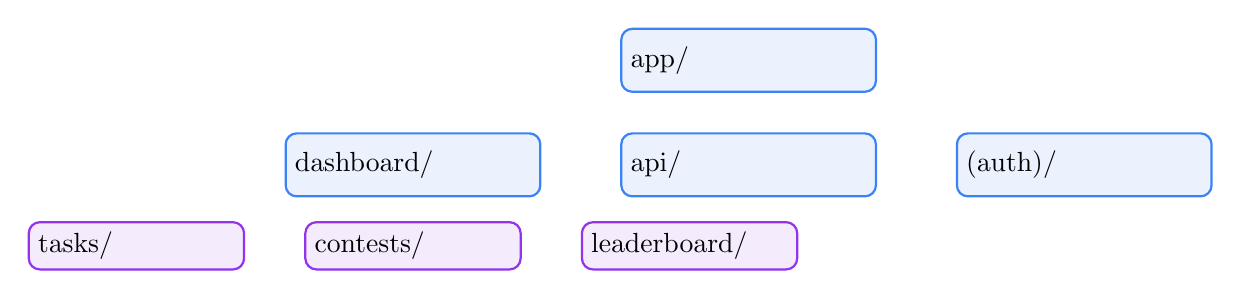
\begin{tikzpicture}[
    folder/.style={rectangle, draw=primary, fill=primary!10, thick, text width=3cm, minimum height=0.8cm, rounded corners},
    file/.style={rectangle, draw=secondary, fill=secondary!10, thick, text width=2.5cm, minimum height=0.6cm, rounded corners},
    arrow/.style={->, >=stealth}
]
    \node[folder] (app) {app/};
    \node[folder, below left=0.5cm and 1cm of app] (dashboard) {dashboard/};
    \node[folder, below=0.5cm of app] (api) {api/};
    \node[folder, below right=0.5cm and 1cm of app] (auth) {(auth)/};
    
    \node[file, below left=0.3cm and 0.5cm of dashboard] (tasks) {tasks/};
    \node[file, below=0.3cm of dashboard] (contests) {contests/};
    \node[file, below right=0.3cm and 0.5cm of dashboard] (leaderboard) {leaderboard/};
\end{tikzpicture}

\section{Component Architecture}

\subsection{Component Hierarchy}

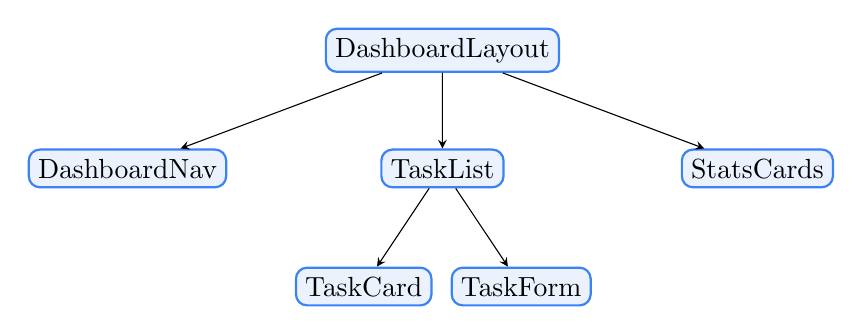
\begin{tikzpicture}[
    level 1/.style={sibling distance=4cm, level distance=1.5cm},
    level 2/.style={sibling distance=2cm},
    component/.style={rectangle, draw=primary, fill=primary!10, thick, rounded corners, text centered},
    edge from parent/.style={draw, ->, >=stealth}
]
    \node[component] {DashboardLayout}
        child {node[component] {DashboardNav}}
        child {node[component] {TaskList}
            child {node[component] {TaskCard}}
            child {node[component] {TaskForm}}
        }
        child {node[component] {StatsCards}};
\end{tikzpicture}

\subsection{State Management}

Momentum uses multiple state management strategies:

\begin{featurebox}{State Management Layers}
\begin{enumerate}
    \item \textbf{Server State} - React Query for API data
    \item \textbf{Client State} - Zustand stores for UI state
    \item \textbf{Form State} - React Hook Form for forms
    \item \textbf{URL State} - Next.js router for navigation state
\end{enumerate}
\end{featurebox}

\section{UI Component Library}

Built on Shadcn/ui and Radix UI primitives:

\begin{table}[h]
\centering
\begin{tabular}{@{}ll@{}}
\toprule
\textbf{Component} & \textbf{Usage} \\ \midrule
Button & Actions and CTAs \\
Card & Content containers \\
Dialog & Modals and overlays \\
Form & Data input \\
Toast & Notifications \\
Badge & Status indicators \\
Progress & Loading states \\
Tabs & Content organization \\
\bottomrule
\end{tabular}
\caption{Core UI components}
\end{table}

\section{Styling System}

\subsection{Tailwind Configuration}

Custom design tokens extend Tailwind's defaults:

\begin{lstlisting}[language=JavaScript, caption=tailwind.config.js]
module.exports = {
  theme: {
    extend: {
      colors: {
        primary: 'hsl(var(--primary))',
        secondary: 'hsl(var(--secondary))',
        accent: 'hsl(var(--accent))',
      },
      animation: {
        'fade-in': 'fadeIn 0.3s ease-in',
        'slide-up': 'slideUp 0.4s ease-out',
      },
    },
  },
}
\end{lstlisting}

% Chapter 6: Deployment
\chapter{Deployment \& DevOps}

\section{Deployment Architecture}

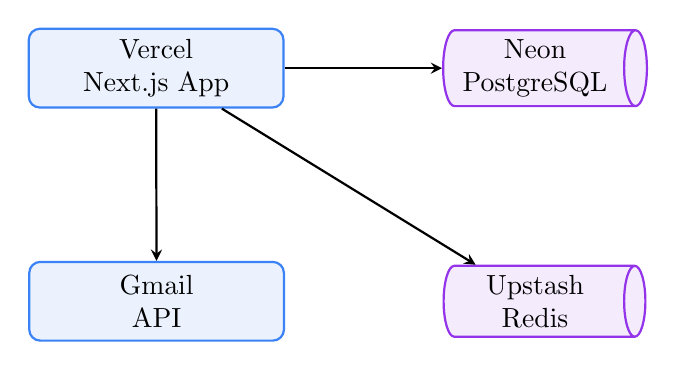
\begin{tikzpicture}[
    node distance=2cm,
    service/.style={rectangle, draw=primary, fill=primary!10, thick, text width=3cm, text centered, rounded corners, minimum height=1cm},
    db/.style={cylinder, draw=secondary, fill=secondary!10, thick, aspect=0.3, text width=2cm, text centered},
    arrow/.style={->, >=stealth, thick}
]
    \node[service] (vercel) {Vercel\\Next.js App};
    \node[db, right=of vercel] (neon) {Neon\\PostgreSQL};
    \node[db, below=of neon] (redis) {Upstash\\Redis};
    \node[service, left=of redis] (email) {Gmail\\API};
    
    \draw[arrow] (vercel) -- (neon);
    \draw[arrow] (vercel) -- (redis);
    \draw[arrow] (vercel) -- (email);
\end{tikzpicture}

\section{Environment Variables}

\begin{lstlisting}[caption=.env.local]
# Database
DATABASE_URL=postgresql://...
DIRECT_URL=postgresql://...

# Auth
BETTER_AUTH_SECRET=...
BETTER_AUTH_URL=http://localhost:3000

# AI
GOOGLE_GEMINI_API_KEY=...

# Redis
UPSTASH_REDIS_REST_URL=...
UPSTASH_REDIS_REST_TOKEN=...

# Email
GMAIL_USER=...
GMAIL_APP_PASSWORD=...

# Storage
UPLOADTHING_SECRET=...
UPLOADTHING_APP_ID=...
\end{lstlisting}

\section{CI/CD Pipeline}

Vercel provides automatic deployments:

\begin{tikzpicture}[
    node distance=1.5cm,
    step/.style={rectangle, draw=success, fill=success!10, thick, text width=4cm, text centered, rounded corners, minimum height=1cm},
    arrow/.style={->, >=stealth, thick}
]
    \node[step] (push) {Git push to main};
    \node[step, below=of push] (build) {Vercel build};
    \node[step, below=of build] (test) {Run tests};
    \node[step, below=of test] (deploy) {Deploy to production};
    \node[step, below=of deploy] (verify) {Health checks};
    
    \draw[arrow] (push) -- (build);
    \draw[arrow] (build) -- (test);
    \draw[arrow] (test) -- (deploy);
    \draw[arrow] (deploy) -- (verify);
\end{tikzpicture}

\section{Monitoring \& Observability}

\begin{featurebox}{Monitoring Stack}
\begin{itemize}
    \item \textbf{Vercel Analytics} - Web vitals and performance
    \item \textbf{PostgreSQL Logs} - Database query performance
    \item \textbf{Redis Monitoring} - Cache hit rates
    \item \textbf{Error Tracking} - Runtime error aggregation
    \item \textbf{Uptime Monitoring} - Service availability checks
\end{itemize}
\end{featurebox}

% Chapter 7: Security
\chapter{Security \& Privacy}

\section{Authentication Security}

Better Auth provides enterprise-grade security:

\begin{itemize}
    \item \textbf{Password Hashing} - Argon2id algorithm
    \item \textbf{Session Management} - Secure, httpOnly cookies
    \item \textbf{CSRF Protection} - Token-based validation
    \item \textbf{Rate Limiting} - Upstash Redis limiter
    \item \textbf{Email Verification} - Required for sensitive actions
\end{itemize}

\section{Data Protection}

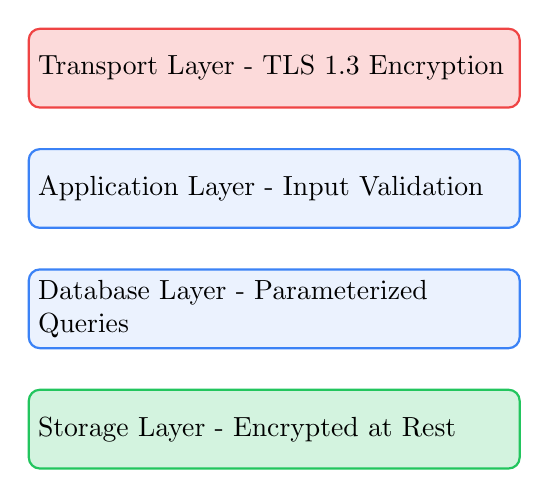
\begin{tikzpicture}[
    layer/.style={rectangle, draw=primary, fill=primary!10, thick, text width=6cm, minimum height=1cm, rounded corners},
    node distance=0.5cm
]
    \node[layer, fill=danger!20, draw=danger] (transport) {Transport Layer - TLS 1.3 Encryption};
    \node[layer, below=of transport] (app) {Application Layer - Input Validation};
    \node[layer, below=of app] (db) {Database Layer - Parameterized Queries};
    \node[layer, below=of db, fill=success!20, draw=success] (storage) {Storage Layer - Encrypted at Rest};
\end{tikzpicture}

\section{Privacy Compliance}

\begin{notebox}
\textbf{GDPR Compliance Features:}
\begin{itemize}
    \item User data export capability
    \item Account deletion with cascade
    \item Cookie consent management
    \item Privacy policy integration
    \item Data retention policies
\end{itemize}
\end{notebox}

% Chapter 8: Performance Optimization
\chapter{Performance Optimization}

\section{Caching Strategy}

Multi-layer caching for optimal performance:

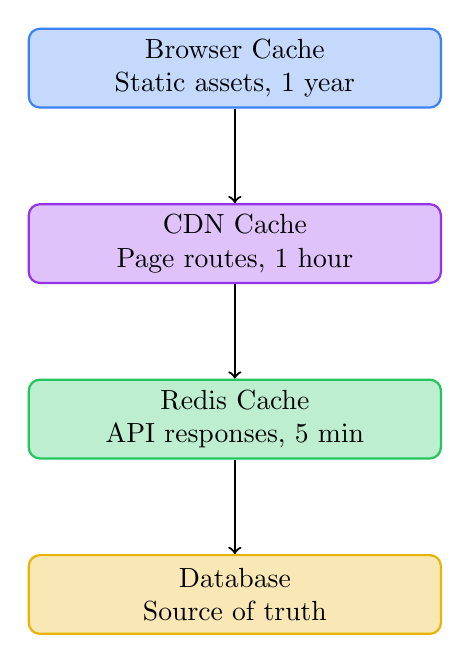
\begin{tikzpicture}[
    node distance=1.2cm,
    cache/.style={rectangle, draw, thick, text width=5cm, minimum height=1cm, rounded corners, text centered}
]
    \node[cache, fill=primary!30, draw=primary] (browser) {Browser Cache\\Static assets, 1 year};
    \node[cache, below=of browser, fill=secondary!30, draw=secondary] (cdn) {CDN Cache\\Page routes, 1 hour};
    \node[cache, below=of cdn, fill=success!30, draw=success] (redis) {Redis Cache\\API responses, 5 min};
    \node[cache, below=of redis, fill=warning!30, draw=warning] (db) {Database\\Source of truth};
    
    \draw[->, thick] (browser) -- (cdn);
    \draw[->, thick] (cdn) -- (redis);
    \draw[->, thick] (redis) -- (db);
\end{tikzpicture}

\section{Database Optimization}

\subsection{Query Optimization}

\begin{lstlisting}[language=SQL, caption=Optimized Query Example]
-- Use indexes and select only needed fields
SELECT 
    t.id, t.title, t.status, t.priority
FROM task t
WHERE 
    t.user_id = $1 
    AND t.status = 'todo'
ORDER BY t.priority DESC, t.due_date ASC
LIMIT 20;
\end{lstlisting}

\subsection{Connection Pooling}

Drizzle ORM with Neon serverless driver handles connection pooling automatically:

\begin{lstlisting}[language=JavaScript]
import { neon, neonConfig } from '@neondatabase/serverless';
import { drizzle } from 'drizzle-orm/neon-http';

neonConfig.fetchConnectionCache = true;
const sql = neon(process.env.DATABASE_URL!);
export const db = drizzle(sql);
\end{lstlisting}

\section{Frontend Performance}

\subsection{Code Splitting}

Next.js automatic code splitting:

\begin{lstlisting}[language=JavaScript, caption=Dynamic Imports]
import dynamic from 'next/dynamic';

const HeavyComponent = dynamic(
  () => import('@/components/heavy-component'),
  { loading: () => <Skeleton /> }
);
\end{lstlisting}

\subsection{Image Optimization}

Next.js Image component with automatic optimization:

\begin{lstlisting}[language=JSX]
<Image
  src="/hero.png"
  alt="Momentum"
  width={1200}
  height={600}
  priority
  placeholder="blur"
/>
\end{lstlisting}

% Chapter 9: Testing
\chapter{Testing Strategy}

\section{Testing Pyramid}

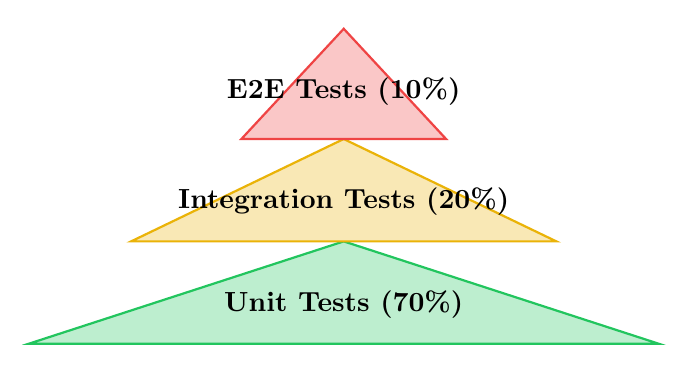
\begin{tikzpicture}
    % Draw pyramid
    \coordinate (apex) at (0,4);
    \coordinate (bottomleft) at (-4,0);
    \coordinate (bottomright) at (4,0);
    
    % Layers
    \filldraw[fill=success!30, draw=success, thick] 
        (bottomleft) -- (bottomright) -- (0,1.3) -- cycle;
    \filldraw[fill=warning!30, draw=warning, thick] 
        (-2.7,1.3) -- (2.7,1.3) -- (0,2.6) -- cycle;
    \filldraw[fill=danger!30, draw=danger, thick] 
        (-1.3,2.6) -- (1.3,2.6) -- (apex) -- cycle;
    
    % Labels
    \node[font=\bfseries] at (0,0.5) {Unit Tests (70\%)};
    \node[font=\bfseries] at (0,1.8) {Integration Tests (20\%)};
    \node[font=\bfseries] at (0,3.2) {E2E Tests (10\%)};
\end{tikzpicture}

\section{Unit Testing}

Example unit test for gamification logic:

\begin{lstlisting}[language=JavaScript, caption=Jest Unit Test]
import { calculateLevel, getPointsForNextLevel } from '@/lib/gamification';

describe('Gamification', () => {
  test('calculates correct level from points', () => {
    expect(calculateLevel(0)).toBe(1);
    expect(calculateLevel(100)).toBe(2);
    expect(calculateLevel(400)).toBe(3);
    expect(calculateLevel(900)).toBe(4);
  });
  
  test('calculates points needed for next level', () => {
    expect(getPointsForNextLevel(1)).toBe(400);
    expect(getPointsForNextLevel(2)).toBe(900);
  });
});
\end{lstlisting}

\section{Integration Testing}

API route testing with Vitest:

\begin{lstlisting}[language=JavaScript, caption=API Integration Test]
import { POST } from '@/app/api/tasks/route';

describe('/api/tasks', () => {
  it('creates task with AI decomposition', async () => {
    const request = new Request('http://localhost:3000/api/tasks', {
      method: 'POST',
      body: JSON.stringify({
        title: 'Build feature',
        description: 'Implement new dashboard',
        dueDate: '2024-12-31',
        priority: 'high',
        estimatedTime: 240,
        aiDecompose: true
      })
    });
    
    const response = await POST(request);
    expect(response.status).toBe(201);
  });
});
\end{lstlisting}

% Chapter 10: Future Enhancements
\chapter{Future Enhancements}

\section{Roadmap}

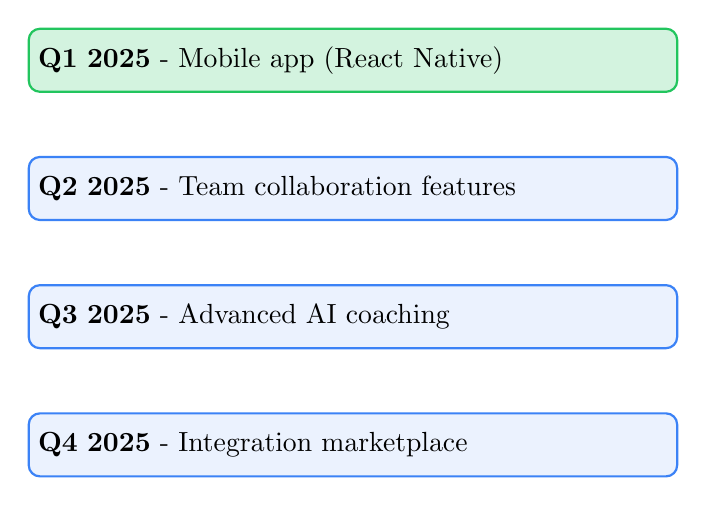
\begin{tikzpicture}[
    node distance=0.8cm,
    phase/.style={rectangle, draw=primary, fill=primary!10, thick, text width=8cm, minimum height=0.8cm, rounded corners}
]
    \node[phase, fill=success!20, draw=success] (q1) {\textbf{Q1 2025} - Mobile app (React Native)};
    \node[phase, below=of q1] (q2) {\textbf{Q2 2025} - Team collaboration features};
    \node[phase, below=of q2] (q3) {\textbf{Q3 2025} - Advanced AI coaching};
    \node[phase, below=of q3] (q4) {\textbf{Q4 2025} - Integration marketplace};
\end{tikzpicture}

\section{Planned Features}

\subsection{Mobile Applications}

Native iOS and Android apps with:
\begin{itemize}
    \item Push notifications for task reminders
    \item Offline mode with sync
    \item Widget support for quick task access
    \item Biometric authentication
\end{itemize}

\subsection{Team Collaboration}

\begin{featurebox}{Team Features}
\begin{itemize}
    \item Shared workspaces and task boards
    \item Team leaderboards and challenges
    \item Manager dashboard for team oversight
    \item Collaborative goal setting
    \item Team productivity analytics
\end{itemize}
\end{featurebox}

\subsection{Advanced AI}

\begin{itemize}
    \item \textbf{Predictive Scheduling} - ML-based optimal time suggestions
    \item \textbf{Personalized Coaching} - Adaptive AI mentor
    \item \textbf{Habit Recognition} - Automatic pattern detection
    \item \textbf{Smart Prioritization} - AI-driven task ordering
\end{itemize}

\subsection{Integration Ecosystem}

Planned integrations:
\begin{itemize}
    \item Calendar: Google Calendar, Outlook, Apple Calendar
    \item LMS: Canvas, Blackboard, Moodle, Google Classroom
    \item Communication: Slack, Discord, Microsoft Teams
    \item Project Management: Jira, Trello, Asana
    \item Health: Apple Health, Google Fit, Fitbit
\end{itemize}

\section{Scaling Considerations}

\subsection{Infrastructure Scaling}

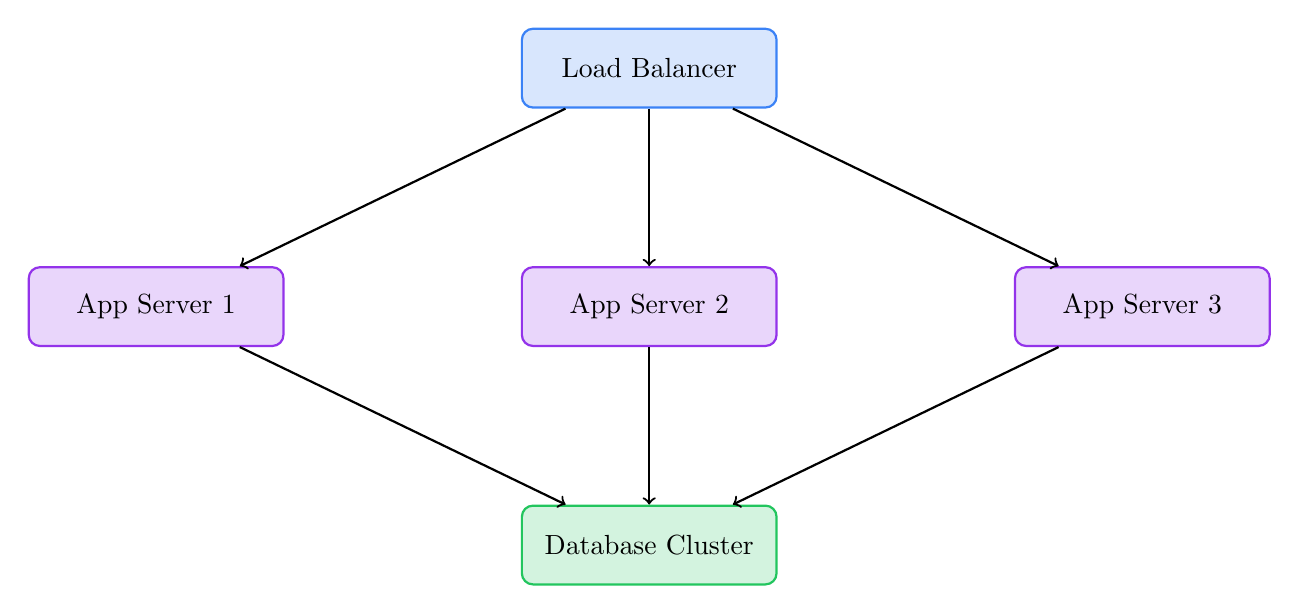
\begin{tikzpicture}[
    node distance=2cm and 3cm,
    component/.style={rectangle, draw, thick, text width=3cm, text centered, rounded corners, minimum height=1cm}
]
    \node[component, fill=primary!20, draw=primary] (lb) {Load Balancer};
    \node[component, fill=secondary!20, draw=secondary, below left=of lb] (app1) {App Server 1};
    \node[component, fill=secondary!20, draw=secondary, below=of lb] (app2) {App Server 2};
    \node[component, fill=secondary!20, draw=secondary, below right=of lb] (app3) {App Server 3};
    \node[component, fill=success!20, draw=success, below=of app2] (db) {Database Cluster};
    
    \draw[->, thick] (lb) -- (app1);
    \draw[->, thick] (lb) -- (app2);
    \draw[->, thick] (lb) -- (app3);
    \draw[->, thick] (app1) -- (db);
    \draw[->, thick] (app2) -- (db);
    \draw[->, thick] (app3) -- (db);
\end{tikzpicture}

\subsection{Database Sharding}

For large-scale deployment:
\begin{itemize}
    \item User-based sharding (shard by user\_id)
    \item Read replicas for query distribution
    \item Eventual consistency for non-critical data
\end{itemize}

% Appendices
\appendix

\chapter{API Quick Reference}

\section{Authentication}
\begin{itemize}
    \item POST /api/auth/signup - Create account
    \item POST /api/auth/login - User login
    \item POST /api/auth/logout - End session
    \item POST /api/auth/reset-password - Password reset
\end{itemize}

\section{Tasks}
\begin{itemize}
    \item GET /api/tasks - List tasks
    \item POST /api/tasks - Create task
    \item PATCH /api/tasks/[id] - Update task
    \item DELETE /api/tasks/[id] - Delete task
\end{itemize}

\section{Contests}
\begin{itemize}
    \item GET /api/contest - List contests
    \item POST /api/contest - Create contest
    \item GET /api/contest/[id] - Contest details
    \item POST /api/contest/[id]/join - Join contest
\end{itemize}

\chapter{Glossary}

\begin{description}
    \item[AI Decomposition] Process of breaking complex tasks into subtasks using AI
    \item[Gamification] Application of game mechanics to increase engagement
    \item[Pomodoro] Time management technique with focused work intervals
    \item[Procrastination Alert] System notification about task avoidance
    \item[Schedule Block] Time-boxed calendar entry for tasks or breaks
    \item[Streak] Consecutive days of task completion
    \item[Wellness Metric] Tracked health and break activities
\end{description}

\chapter{Contributing Guidelines}

\section{Development Setup}

\begin{lstlisting}[language=bash, caption=Local Setup Commands]
# Clone repository
git clone https://github.com/AyushPandey003/momentum-app.git
cd momentum-app

# Install dependencies
pnpm install

# Setup environment
cp .env.example .env.local
# Fill in environment variables

# Run database migrations
pnpm drizzle-kit push

# Start development server
pnpm dev
\end{lstlisting}

\section{Code Style}

\begin{itemize}
    \item \textbf{TypeScript} - Strict mode enabled
    \item \textbf{ESLint} - Follow Next.js recommended config
    \item \textbf{Prettier} - Automatic code formatting
    \item \textbf{Commit Convention} - Conventional Commits standard
\end{itemize}

\section{Pull Request Process}

\begin{enumerate}
    \item Fork the repository
    \item Create a feature branch: \texttt{git checkout -b feature/amazing-feature}
    \item Commit changes: \texttt{git commit -m 'feat: add amazing feature'}
    \item Push to branch: \texttt{git push origin feature/amazing-feature}
    \item Open a Pull Request with detailed description
\end{enumerate}

% Conclusion
\chapter*{Conclusion}
\addcontentsline{toc}{chapter}{Conclusion}

Momentum represents a comprehensive approach to modern productivity management, combining cutting-edge AI technology with proven time management techniques and engaging gamification mechanics. The platform's architecture is designed for scalability, performance, and extensibility, making it suitable for both individual users and team deployments.

\vspace{0.5cm}

The integration of real-time competitive features, intelligent task decomposition, and wellness monitoring creates a holistic productivity ecosystem that addresses not just task completion, but overall well-being and sustained motivation.

\vspace{0.5cm}

As the platform continues to evolve, the roadmap focuses on expanding integration capabilities, enhancing AI intelligence, and building collaborative features that make productivity engaging and social.

\vspace{1cm}

\begin{center}
\Large\textbf{Build Unstoppable Momentum}
\end{center}

% Contact and Resources
\chapter*{Resources \& Contact}
\addcontentsline{toc}{chapter}{Resources \& Contact}

\section*{Project Links}

\begin{itemize}
    \item \textbf{GitHub Repository:} \url{https://github.com/AyushPandey003/momentum-app}
    \item \textbf{Live Demo:} \url{https://momentum-app.vercel.app}
    \item \textbf{Documentation:} \url{https://momentum-docs.vercel.app}
\end{itemize}

\section*{Author Contact}

\begin{itemize}
    \item \textbf{Name:} Ayush Pandey
    \item \textbf{GitHub:} \faGithub\ \href{https://github.com/AyushPandey003}{AyushPandey003}
    \item \textbf{Email:} \faEnvelope\ ayush.pandey@example.com
\end{itemize}

\section*{License}

This project is licensed under the MIT License. See LICENSE file for details.

\vfill

\begin{center}
\textit{Generated on \today}
\end{center}

\end{document}
